% PLANTILLA APA7
% Creado por: Isaac Palma Medina
% Última actualización: 25/07/2021
% @COPYLEFT

% Fuentes consultadas (todos los derechos reservados):  
% Normas APA. (2019). Guía Normas APA. https://normas-apa.org/wp-content/uploads/Guia-Normas-APA-7ma-edicion.pdf
% Tecnológico de Costa Rica [Richmond]. (2020, 16 abril). LaTeX desde cero con Overleaf (1 de 3) [Vídeo]. YouTube. https://www.youtube.com/watch?v=kM1KvHVuaTY Weiss, D. (2021). 
% Formatting documents in APA style (7th Edition) with the apa7 LATEX class. https://ctan.math.washington.edu/tex-archive/macros/latex/contrib/apa7/apa7.pdf @COPYLEFT

%+-+-+-+-++-+-+-+-+-+-+-+-+-++-+-+-+-+-+-+-+-+-+-+-+-+-+-+-+-+-++-+-+-+-+-+-+-+-+-+

% Preámbulo
\documentclass[stu, 12pt, letterpaper, donotrepeattitle, floatsintext, natbib, helv]{apa7}
\usepackage[utf8]{inputenc}
\usepackage{comment}
\usepackage{marvosym}
\usepackage{graphicx}
\usepackage{float}
\usepackage[normalem]{ulem}
\usepackage[spanish]{babel} 
%\usepackage{titling}
\let\apasubparagraph\subparagraph
\let\subparagraph\paragraph
\usepackage[compact]{titlesec}
\let\subparagraph\apasubparagraph
\usepackage{hyperref}
\selectlanguage{spanish}
\useunder{\uline}{\ul}{}
\newcommand{\myparagraph}[1]{\paragraph{#1}\mbox{}\\}
\graphicspath{{./images/}}
\titleformat{\section}{\normalfont\large\bfseries}{\thetitle. \quad }{0pt}{}[{ \titlerule[0.8pt]}]
\titleformat{\subsection}{\normalfont\bfseries}{}{}{}[]

% Portada

\begin{document}
\begin{titlepage}
    \centering
    \vfill
    \LARGE Laboratorio \#3\\
    \vskip2cm
    \large Diego Quirós Artiñano \\
    Universidad Nacional de Costa Rica \\
    EIF-202: Soporte Técnico \\ 
    Carolina Gómez Fernández \\
    17 de abril, 2022 \\
    \vfill
    
\includegraphics[width = 0.4\textwidth]{../../../UNAImage/UNA.png} \\
    \vfill
    \vfill
    % (autores separados, consultar al docente)
    % Manera oficial de colocar los autores:
    %\author{Autor(a) I, Autor(a) II, Autor(a) III, Autor(a) X}
\end{titlepage}

% Índices
\pagenumbering{roman}
    % Contenido
\addto\captionsspanish{
    \renewcommand*\contentsname{\largeÍndice}
}
\tableofcontents
\setcounter{tocdepth}{2}
\newpage
    % Figuras
\renewcommand{\listfigurename}{\largeÍndice de fíguras}
\listoffigures
\newpage
    % Tablas
%\renewcommand{\listtablename}{\largeÍndice de tablas}
%\listoftables
%\newpage

% Cuerpo
\pagenumbering{arabic}

%------------------------------------------------------------------------------------
\section*{Introducción}
\phantomsection
\addcontentsline{toc}{section}{Introducción}
En este documento se va a investigar sobre varias compuertas lógicas y después se van a hacer circuitos con estas compuertas lógicas.
%------------------------------------------------------------------------------------
\section*{Investigación}
\phantomsection
\addcontentsline{toc}{section}{Investigación}

\subsection*{La compuerta negadora NOT 7404}
\addcontentsline{toc}{subsection}{La compuerta negadora NOT 7404}
Según \cite{CompuertaLogicaNOT}, es una compuerta lógica con "el propósito es producir una salida inversa o contraria a su entrada." El activo termina como inactivo y viceversa.

\subsection*{La compuerta multiplicadora AND 7408}
\addcontentsline{toc}{subsection}{La compuerta multiplicadora AND 7408}
Según \cite{CompuertaLogicaAND}, es la compuerta "conocida como "todo o nada." En el Álgebra de Boole se representa por una multiplicación." Todas las entradas son activas para que termine como activa o termina como inactiva, como en la multiplicación normal, si algo se multiplica por cero entonces todo es 0. La versión de 7408, es la compuerta AND pero con solo dos entradas.

\subsection*{La compuerta sumadora OR 7432}
\addcontentsline{toc}{subsection}{La compuerta sumadora OR 7432}
Según \cite{CompuertaLogicaOR}, es la compuerta "de "cualquiera o todo". Su expresión en el Álgebra de Boole es representada por una suma." Si algo es activo entonces todo es activo, sino entonces es inactivo (solo si todo es inactivo). La expresión es de A+B = Q, donde A y B son preposiciones y Q el resultado. La versión 7432, es la compuerta OR con solo dos entradas.
%------------------------------------------------------------------------------------
\section*{Circuitos}
\phantomsection
\addcontentsline{toc}{section}{Circuitos}

\begin{figure} [H]
    \centering
    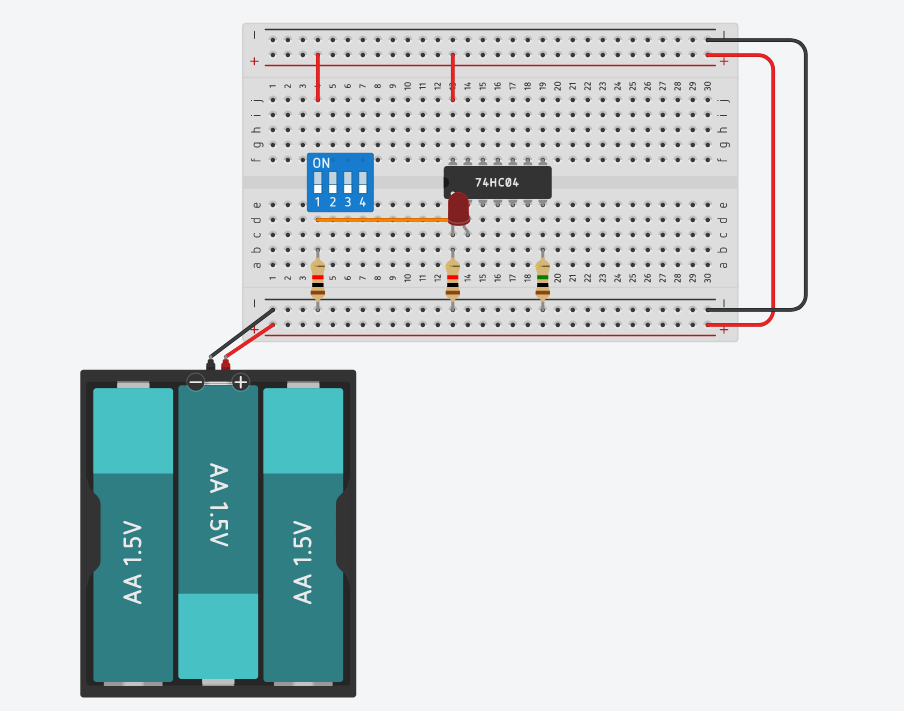
\includegraphics[width=1\textwidth]{Circuito1.png}
    \caption{Circuito 1 con la compuerta NOT, \cite{circuits}}
    \label{fig:NOT}
\end{figure}

\begin{figure} [H]
    \centering
    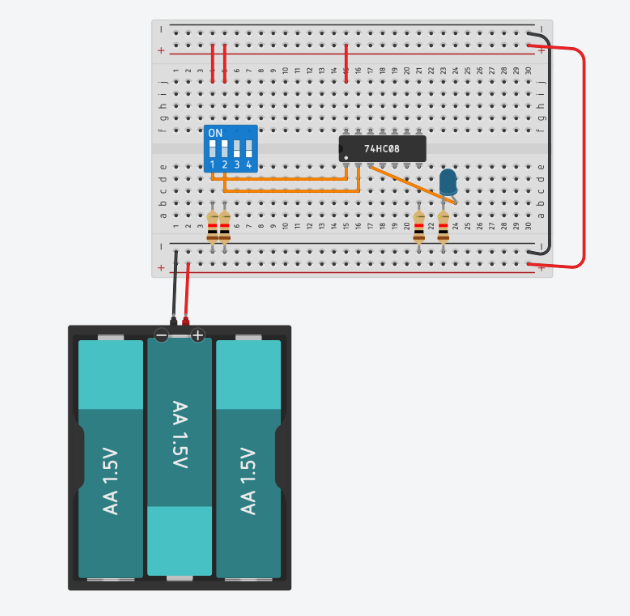
\includegraphics[width=1\textwidth]{Circuito2.png}
    \caption{Circuito 2 con la compuerta AND, \cite{circuits}}
    \label{fig:AND}
\end{figure}

\begin{figure} [H]
    \centering
    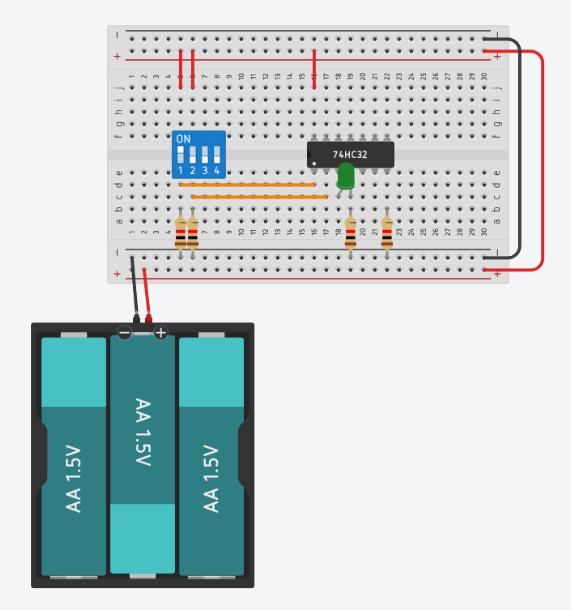
\includegraphics[width=1\textwidth]{Circuito3.png}
    \caption{Circuito 3 con la compuerta OR, \cite{circuits}}
    \label{fig:OR} 
\end{figure}

\begin{figure} [H]
    \centering
    \includegraphics[width=1\textwidth]{Brilliant Elzing-ROttis.png}
    \caption {Todos los circuitos, \cite{circuits}}
    \label{fig:ALL}
\end{figure}

Los tres circuitos no son muy complicados, son el básico power y ground en todos los componentes, con resistencias para que no se quiebre nada, meter el output de los \textit{DIP switches} al input de la compuerta lógica. Pero cada uno cumple un propósito, el NOT se podría usar para prender luces cuando no hay luz por ejemplo usando una photoresistencia, el AND podría ser para prender algo con mucho cuidado asegurandose que todo lo que tiene que prenderse está prendido (como en las peliculas que tienen a dos personas con llaves para prender una bomba nuclear), y el OR se puede usar como para esas secciones en las casas que se pueden prender con varios \textit{switches}.
%----------------------------------------------------------------------------------------------------------------------------------------------------------------------
\section*{Conclusión}
\phantomsection
\addcontentsline{toc}{section}{Conclusión}

En este laboratorio se aprendió sobre compuertas lógicas y se investigó sobre la NOT, AND y OR. Se generaron circuitos para ejemplificar cada uno de ellos y se discute sobre el posible uso de cada uno de ellos.

\newpage
% Referencias
\renewcommand\refname{\large\textbf{Referencias}}
\bibliography{ref}

\end{document}